\documentclass[%
	%draft,
	%submission,
	%compressed,
	final,
	%
	%technote,
	%internal,
	%submitted,
	%inpress,
	%reprint,
	%
	%titlepage,
	notitlepage,
	%anonymous,
	narroweqnarray,
	inline,
	twoside,
        %invited,
	]{ieee}

\newcommand{\latexiie}{\LaTeX2{\Large$_\varepsilon$}}

\begin{document}

%----------------------------------------------------------------------
% Title Information, Abstract and Keywords
%----------------------------------------------------------------------
\title{Android Synchronization Manager}

\author{Parikshit Ghodake, Imran Ahmed, Akshay Khole, Muneeb Shaikh \\
Department of Computer Engineering, JSCOE \\
University of Pune\\
\{parikshitghodake, iahmed213, akshay2009ark, iammuneeb\}@gmail.com
}

\maketitle               

\begin{abstract} 
Recent developments in mobile computing has increased number of devices with 
software platform as Android. Synchronization with any server is now basic need of 
all mobile devices.
The current scenario in synchronization of Android based mobile devices is that it 
insists users to send information to be backed up to Google servers. Once this 
information is present with Google, they have the right to sell/use that data in 
any way they want according to their “Terms of Service”. This hampers the users’ 
privacy. So to overcome this problem, a offline synchronization manager is 
required. In this paper, we proposed an approach to synchronize Android based 
devices offline.
Usually, when android mobiles are shipped, manufacturers provide an application for 
taking backup of data. But almost always, this application is not cross platform 
compatible and in most cases, not available for installation on linux machines. 
Android being an open source operating system and running on a linux kernel, it is 
but necessary that such a backup tool should be developed. The paper tries to 
address this issue and develop a solution for the same.
\end{abstract}

\begin{keywords}
Data Synchronization, SyncML
\end{keywords}

%----------------------------------------------------------------------
% SECTION 1: Introduction to Android, synchronization
%----------------------------------------------------------------------
\section{Introduction}

\PARstartCal
Android is a software stack for mobile devices that includes an operating system, 
middleware and key applications. The Android SDK provides the tools and APIs 
necessary to begin developing applications on the Android platform using the Java 
programming language. Android has some of the following features as:

\begin{itemize}
\item Application framework enabling reuse and replacement of components
\item Dalvik virtual machine optimized for mobile devices
\item Integrated browser based on the open source WebKit engine
\item Optimized graphics powered by a custom 2D graphics library; 3D graphics based on the OpenGL ES 1.0 specification (hardware acceleration optional)
\item SQLite for structured data storage
\item Media support for common audio, video, and still image formats (MPEG4, H.264, MP3, AAC, AMR, JPG, PNG, GIF)
\item GSM Telephony (hardware dependent)
\item Bluetooth, EDGE, 3G, and WiFi (hardware dependent)
\item Camera, GPS, compass, and accelerometer (hardware dependent)
\item Rich development environment including a device emulator, tools for debugging, memory and performance profiling, and a plugin for the Eclipse IDE
\end{itemize}

Android relies on Linux version 2.6 for core system services such as security, 
memory management, process management, network stack, and driver model. The kernel 
also acts as an abstraction layer between the hardware and the rest of the software 
stack. The Android software stack can be illustrated by the following diagram:

\begin{figure}[h]
 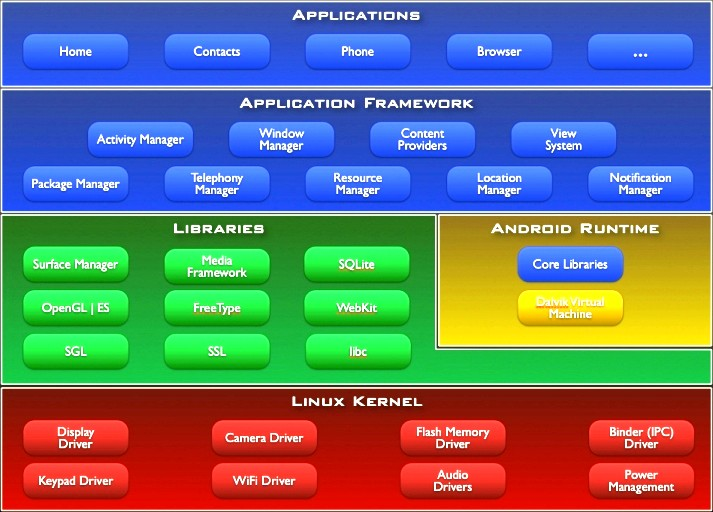
\includegraphics[height= 100mm, width= 0.5\textwidth]{images/system-architecture}
 \caption{System Architecture of Android}
 \centering
\end{figure}

Every Android application runs in its own process, with its own instance of the 
Dalvik virtual machine. Dalvik has been written so that a device can run multiple 
VMs efficiently. The Dalvik VM executes files in the Dalvik Executable (.dex) 
format which is optimized for minimal memory footprint. The VM is register-based, 
and runs classes compiled by a Java language compiler that have been transformed 
into the \texttt{.dex} format by the included "dx" tool. The Dalvik VM relies on 
the Linux kernel for underlying functionality such as threading and low-level 
memory management.
\\

\textbf{Data synchronization} is the process of establishing consistency among data 
from a source to a target data storage and vice versa and the continuous 
harmonization of the data over time. It is fundamental to a wide variety of 
applications, including file synchronization and mobile device synchronization.

Data synchronization is the process of making two sets of data look identical:

\begin{figure}[h]
 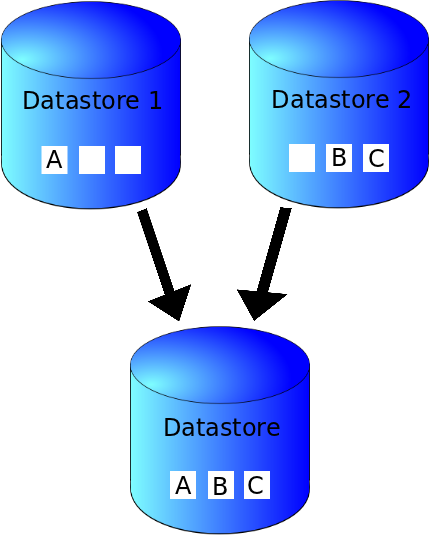
\includegraphics[height= 100mm, width= 0.5\textwidth]{images/data-sync}
 \caption{Data Synchronization}
 \centering
\end{figure}

All mobile devices – handheld computers, mobile phones, pagers, laptops – need to 
synchronize their data with the server where the information is stored. This 
ability to access and update information on the fly is key to the pervasive nature 
of mobile computing. Yet, today, almost every device uses a different technology 
for performing data synchronization.

By definition, mobile users are not always connected to a network and its stored 
data.Users retrieve data from the network and store it on the mobile device, where 
they access and manipulate the local copy of the data. Periodically, users 
reconnect with the network to send any local changes back to the networked data 
repository. Users also have the opportunity to learn about updates made to the 
networked data while the device was disconnected. Occasionally, they need to 
resolve conflicts among the updates made to the networked data. This reconciliation 
operation – where updates are exchanged and conflicts are resolved – is known as 
data synchronization.

The data synchronization protocol would synchronize networked data with many
different devices, including handheld computers, mobile phones, automotive 
computers, and desktop PCs. A user could access and manipulate the same set of data 
from different devices. For example, a user could read e-mail from either a 
handheld or a mobile phone, and still maintain a consistent, updated record of 
which messages had been read.

%----------------------------------------------------------------------
% SUB-SECTION 1.1: Main contribution of this paper
%----------------------------------------------------------------------
\subsection{Main contribution of this paper}
In this paper, we propose an approach to an offline Android synchronization 
manager, developed to address the issues of privacy when users need to synchronize 
their data. AndroSync brings a concept of offline synchronization for android 
devices. Offline synchronization means syncing data from Android phone to a desktop 
pc means that do not require use to send personal information to any third party.

Offline means of synchronization are syncing over bluetooth, USB data cable or if 
possible using WI-FI. This means user does not need to be connected to the internet 
for backing up data. In the primary stages, this project can be used as a backup 
tool. It can be divided into the client and the server module. The client module is 
an android application where as the server module is a desktop application. The 
client module has the task of accessing all the data that is essential and send 
that data to the server by means of bluetooth or USB or WiFi.

The server , on the other hand which constantly keep listening to requests from 
bluetooth devices. As soon as a devices requests connection, a common handshaking 
procedure can be started and then the two devices can be paired for further 
communication. 

once the two devices are paired, the server can start receiving data from the 
client. The main duty of the server is to maintain a record of all data received. 
also according to timestamp on incoming data, the data should be sorted and stored. 
in case of SMS, the messages can be categorized according to the name of the sender/
receiver. 

% EDITING DONE TILL HERE ONLY

%----------------------------------------------------------------------
% SECTION II: The Document Life-Cycle
%----------------------------------------------------------------------
\section{The Document Life-Cycle}

Each document to be published, regardless of whether it is destined to
be a journal article or a conference paper, goes through a certain
life-cycle. At each stage of the life-cycle, there are different
formatting needs. This may be summarized as follows:
\begin{description}
\item[Draft:] The first stage in the life-cycle is the draft stage.
    This is when the author is initially writing and editing the 
    manuscript. The formatting of the document should help the author 
    with this task. For example, the main text should be
    double-spaced, the margins should be wide enough to allow written
    comments, and a date-and-time stamp should be placed on each page to 
    help with version control.
\item[Internal Review:] After the draft version is finalized,
    the next stage in the life-cycle might be to give the paper
    to one or more colleagues for review. This stage is an internal review
    process, as opposed to the formal review done upon submission
    to the IEEE (see the next stage). Suggestions and 
    criticism at this stage can very much improve the quality of the 
    paper and can save much time in getting the paper 
    published. The formatting for an internal review is fairly flexible. 
    One requirement is that the paper contain a phrase to the effect that
    the document is preliminary and should not be circulated without
    permission of the author(s).  This can appear in the header or footer of
    the paper, for example.
\item[Submission for Review:] The next stage in the life-cycle is to 
    submit the paper to the IEEE for formal review by anonymous reviewers. 
    This review requires that the paper be formatted differently. In some 
    cases, the title of the paper, and especially the authors' names, 
    must be printed on a separate title page to ensure anonymity of the
    authors. Double-spacing of the main text is usually required, but not 
    time stamps, and so forth.
\item[Initial Distribution:] While the document is submitted or 
    ``in-press,'' it is desirable to be able to distribute the 
    preliminary version (e.g., on the world-wide-web) for the 
    benefit of other researchers. This, once again, will stipulate a 
    different format. The paper should indicate that it is
    ``submitted'' or ``in-press,'' and is not the final version, to 
    avoid confusion between the preliminary and eventual printed
    versions. The date is added on each page to further distinguish this
    from the final version.
\item[Final Form:] The IEEE uses its own software to format journal
    papers. The ``final'' mode of the proposed macro package will
    approximate the style of the published paper as closely as possible.
    This allows the researcher to estimate page lengths, and to 
    appropriately break equations and scale figures and tables. Perhaps 
    if a standard set of macro packages is developed, the IEEE may 
    eventually adopt it, and then the final-mode would be exactly 
    what is published!

    For IEEE conferences, the author may (and often must) provide a
    camera-ready formatted copy of the paper. In this case, the 
    ``final'' mode of the macro package produces \emph{exactly} what 
    is published.
\item[Submission for Publishing:] After the paper is accepted,
    and all the final corrections are made, it must be submitted for 
    publishing. To submit a paper to an IEEE conference, the format of 
    the paper is defined by the specifications used in the ``Final Form'' 
    stage of the life-cycle. However, if the paper is to be submitted
    to a journal, there are different formatting requirements for the
    submitted document.
\item[Final Distribution:] After the paper is published, it is
    beneficial to have an electronic version of the paper
    (e.g., for distribution on the world-wide-web). This final
    version should have correct page numbers, the IEEE copyright 
    information, the volume and issue number of the journal, and so forth.
\end{description}

Clearly, it is cumbersome to \emph{manually} re-format a paper for all
the stages of its life-cycle. We believe that a better solution is to
use macro packages for individual text-processing systems which can
automatically format a paper to certain specifications.  The format of
the paper is automatically changed by changing a single parameter.
This is not a dream! This has all been implemented for one
text-processing system (see Section~\ref{sec:latex}), and our hope is
that various readers and proponents of different text-formatting
systems will volunteer to implement these specifications for their
favorite text formatter. The entire research community will benefit
from these efforts.

%----------------------------------------------------------------------
% SECTION III: Specifications
%----------------------------------------------------------------------
\section{Specifications}

In this section, we give specifications which we feel must be
satisfied by a macro package to aid a researcher in preparing papers
for publication. We have followed this list very closely when writing
the example package \texttt{ieee.cls}.

%----------------------------------------------------------------------
\subsection{Draft Manuscript}

The draft mode is the format used while the author writes the manuscript. 
Its main characteristics are:
\begin{itemize}
\item Double spacing, single-column, and acceptably wide margins to allow room for comments and proofreaders' marks.
\item A date-and-time stamp on each page to document the time of the
      printing for help with version control.
\item When figures belong to the manuscript, the author may switch
      among the basic options:
      \begin{enumerate}
      \item Figures are not printed, but the appropriate space is
            left in the manuscript.
      \item Figures are not printed, and the captions are
            included at the marked places with a small empty space.
      \item Figures are inserted into the manuscript.
      \item Figures are inserted one after the other at the end of the
            manuscript. 
      \item Figures are inserted, each on a separate page, at the end of the
            manuscript. 
      \end{enumerate}
\end{itemize}

%----------------------------------------------------------------------
\subsection{Internal Review}
The formatting requirements for an internal review are fairly loose.
The following are suggestions:
\begin{itemize}
\item The following text should be included:
      ``Preliminary version for evaluation: Please do not circulate 
      without the permission of the author(s)''
\item The figures should be included in the text, rather than at the
      end of the document. 
\item The text should be double-spaced, single-column, with wide enough 
      margins to allow for reviewers' corrections.
\item The date should be added to the header of each page. 
\end{itemize}

%----------------------------------------------------------------------
\subsection{Submission for IEEE Formal Review}
\label{sec:review}

The following are desirable for submission to the IEEE:
\begin{itemize}
\item The printout would obligatorily be double-spaced, single-column.  
\item The figures should be placed at the end of the paper and should
      be identical to the figures to be submitted for publication if
      the paper is accepted.
\item As some of the Transactions require a separation of the title
      page and the text to provide anonymity, this should be an
      option. 
\item The date of submission should be added on the title page 
      and the second page if a separate title page is generated.
\end{itemize}

%----------------------------------------------------------------------
\subsection{Transactions-like Printing for Evaluation and Length
Measurement}

This format should follow as precisely as practicable the format of the 
journal.

%----------------------------------------------------------------------
\subsection{Submission for Publication in a Journal}

This could be nearly identical to the case in
Section~\ref{sec:review}.  A mark should be placed in the text to show
about where each figure should go.  Figures may optionally be printed
at a larger scale to allow better photographic reproduction.  The date
of submission and possibly the editor's paper number should be added.

%----------------------------------------------------------------------
\subsection{Camera-ready Form for Conference Submission}

This is the only format that has a very strict and exactly defined
layout.  This layout will be defined separately for each conference,
on the basis of the its author's guide.

%----------------------------------------------------------------------
\subsection{Electronic Distribution (Initial and Final)}

A hardcopy or electronic version of the paper can be useful for
distribution during various stages in its life-cycle, but improper
information in this distributed form can lead to misunderstanding.
The format should provide some specific information.
\begin{itemize}
\item If the paper is currently submitted for review, the
      text ``Submitted to (journal or conference name) for
      publication,'' along with the date, should appear on the title
      page.  
\item If the paper has been accepted for publication, but is not
      yet printed, the text ``Accepted for publication by (journal or
      conference name), (in-press)'' should appear. 
\item In addition, for both of the above situations, the following text 
      should be included: ``Preliminary version: Please do not circulate 
      without the permission of the author(s).''
\item If the version is a reprint, the 
      text ``Reprinted from (journal or conference name)'' should be 
      included. Additionally, the page numbers should match the printed
      version, and the volume number, issue number and IEEE copyright 
      information should be included. 
\item To facilitate the paper's distribution on the world-wide-web,
      the height should be set 
      in a way that it can be printed both on A4 and U.S. letter-size paper. 
      A ``full'' A4 page cannot usually be printed in the United 
      States; the top lines will be missing. 
\end{itemize}
This form should allow a lot of freedom, such as one- or two-column
formatting, the inclusion of a cover page, and so on.

%----------------------------------------------------------------------
% SECTION IV: The LaTeX2e Class
%----------------------------------------------------------------------
\section{The \latexiie\ Class}
\label{sec:latex}

One text-formatting package in common use by researchers is the
\latexiie\ system~\cite{lamport}. Some of its features include a very
flexible macro capability, excellent formatting of mathematical
equations, seamless integration of text into graphics (using the
\texttt{psfrag.sty} package; see~\cite{goossens}), and affordable
price (it's free!).

Documents formatted with \latexiie\ must belong to a certain ``class.''
A class file is a set of macros which tells \latexiie\ how to format
the document. For example, the standard classes which are available
include an article class, a report class, a book class and a letter
class.

For the purpose of writing IEEE papers, we have developed a special
\latexiie\ ``class'' file. Users of \LaTeX\ probably know about
\texttt{IEEEtran.sty}, written by Murray and Balemi. This style was 
originally devised for evaluation and length measurement, but it is
close to meeting some of the above desires. It was written for the
now-obsolete \LaTeX 2.09, and has been modified for \latexiie\ by
N\"{u}chter. The latter, called \texttt{IEEEtran.cls}, may be found on
the IEEE world-wide-web site.  It implements much of the functionality
required for the ``Final Form'' stage of the document life-cycle. We
found it helpful as a starting point for this project. Our modified
version, called \texttt{ieee.cls}, satisfies all of the requirements
for each stage of the document life-cycle.

\subsection{Choosing the Paper's Style}

Documents written for \latexiie\ are written as plain text. The
\latexiie\ system converts the text into formatted pages. To tell
\latexiie\ how to format your document, certain commands need to be
entered into the text.

The \texttt{ieee.cls} class file makes this very easy.  The first line
of your document needs to specify a command of the form
\begin{verbatim}
  \documentclass[main-mode,
                 sub-mode,
                 misc-options]{ieee}
\end{verbatim}
where one ``main-mode'' is chosen from the following:
\begin{description}
\item[\texttt{draft}] Double-spaced, single-column, with date and time
     stamp.
\item[\texttt{submission}] Double-spaced, suitable for submitting the
     paper for review, or for submitting the paper for publishing.
\item[\texttt{compressed}] Same as ``submission,'' only single-spaced.
     This is suitable for archival, internal review, and for some 
     conference proceedings. 
\item[\texttt{final}] For IEEE journals, this mode approximates the
     journal's final form. For IEEE conferences, it formats
     the paper for a camera-ready printout.
\end{description}
The optional ``sub-mode'' is chosen from the following:
\begin{description}
\item[\texttt{internal}] The internal sub-mode can modify either the
    ``submission,'' 
    ``compressed,'' or ``final'' modes. It changes the header to notify 
    the reader that this is an evaluation preprint, and not to be
    distributed. 
\item[\texttt{submitted}] The submitted sub-mode can modify either the
    ``compressed'' or ``final'' modes. It changes the header to notify 
    the reader that this paper has been submitted to a certain journal 
    for publication, and that it is not to be distributed.
\item[\texttt{inpress}] The inpress sub-mode is similar to the submitted 
    sub-mode. It can modify either the ``compressed'' or ``final'' modes. 
    It changes the header to notify the 
    reader that this paper has been accepted by a certain journal for 
    publication, but that it has not yet been published. It specifies that 
    the paper is not to be distributed.
\item[\texttt{reprint}] The reprint sub-mode can modify only the ``final''
    mode. It changes the header to state that the paper is reprinted
    from a certain journal. It includes proper page numbers, IEEE
    copyright information and the IEEE log number.
\item[\texttt{technote}] When used in combination with ``final,''
    this sub-mode produces a two-column technical note.
\end{description}
The optional ``misc-options'' are chosen from the following:
\begin{description}
\item[\texttt{titlepage/notitlepage}] The titlepage option causes a
    separate title page to be produced. The notitlepage option 
    (default) does not produce a separate title page.
\item[\texttt{anonymous}] By default, all author information is included
    in the typeset paper.
    However, if the ``anonymous'' option is selected, author information
    is omitted from the paper (except for on the optional title page).
    Author information is omitted from the title line on the first
    page of the paper and from the header on all pages. The author's
    affiliation is omitted from the first page, and the author's 
    biography is also omitted. Anonymity may be required when
    submitting a paper for review.
\item[\texttt{invited}] If the paper is an invited paper (as this
    one is), the ``invited'' option prints \emph{(Invited Paper)} under the 
    authors' names on the first page of the paper.
\item[\texttt{9pt,10pt,11pt,12pt}] You may manually choose the paper's 
    type size.
    You should not need to do this since the ``correct'' size is
    automatically chosen. However, if you want, you may use these to
    change the type size of the main text. (``9pt'' is a bit of a hack
    to retain backward-compatibility.)
\item[\texttt{narroweqnarray}] This fixes a \LaTeX\ bug. The
    spacing around the ``='' sign in equation arrays is changed 
    to be the same as in displayed math.  
\item[\texttt{inline}] Compresses the horizontal spacing of in-text
    math equations. The authors think that the resulting equations
    look better than those normally produced by \latexiie.
\end{description}

Already we can see the power of \texttt{ieee.cls}. By changing a
single parameter in the first line of the document, the user can
change the entire format of the paper!

\subsection{Plug-Ins}

The main \texttt{ieee.cls} file specifies the formatting required for
a generic IEEE journal. However, some journals have their own
formatting particularities. For example, journals of the IEEE Signal
Processing Society have centered figure captions, and all other
journals have left-justified captions. Journals of the IEEE Computer
Society are formatted very differently from journals of all other
societies. Furthermore, each conference has its own style.

Rather than burdening the main \texttt{ieee.cls} file with the
definitions required for each journal, we have placed this task on
small ``plug-in'' files designed to work with \texttt{ieee.cls}. For
example, to format a document for the IEEE Transactions on Computers,
specify (after the \verb|\documentclass| command):
\begin{verbatim}
  \usepackage{ieeetc}
\end{verbatim}
Plug-in files are also used to format papers for conferences. The 
main mode of the paper should be ``final,'' and the 
conference style-file should be loaded. For example,
\begin{verbatim}
  \usepackage{ieeeimtc}
\end{verbatim}
specifies the style needed for the IEEE Instrumentation and
Measurement Technology Conference.

At the moment, plug-in files exist for almost all of the IEEE journals
(see the world-wide-web site mentioned in the Conclusion for
up-to-date information on which are supported), but only a few
conferences.  However, as the use of the \texttt{ieee.cls} package
increases, additional plug-ins will be created.

\subsection{More Definitions}

In addition to specification of the modes and options for the paper,
several more things need to be defined. For a regular IEEE journal
submission, define the journal name in the form
\begin{verbatim}
  \journal{IEEE Trans.\ Something}
\end{verbatim}
The journal name is used to compose the header for each page.  To add
any other information after the journal name, use \verb|\titletext|.
For example, to indicate the editor's manuscript number on a preprint,
you would type something like
\begin{verbatim}
  \titletext{, TN\#9999.}
\end{verbatim}

The date is printed in the header for certain combinations of document
options (e.g., for the submission mode). If you would like to pre-date
or post-date the article, type, for example,
\begin{verbatim}
  \renewcommand{\today}{July 4, 1776}
\end{verbatim}
To specify the IEEE copyright information on the first page of a
reprint, type
\begin{verbatim}
  \ieeecopyright{xxx--xxxx/97\$10.00 
    \copyright\ 1997 IEEE}
\end{verbatim}

Reprints also contain either an ``IEEE log number,'' a ``publisher
item identifier,'' or similar publishing information in the lower left
column on the first page. This can be entered as
\begin{verbatim}
  \lognumber{xxxxxxx}
\end{verbatim}
or
\begin{verbatim}
  \pubitemident{S xxxx--xxxx(97)xxxxx--x}
\end{verbatim}
or
\begin{verbatim}
  \loginfo{Manuscript received... }
\end{verbatim}
To specify the first page of a reprint of a paper beginning on page 
103 of a journal, you would type
\begin{verbatim}
  \firstpage{103}
\end{verbatim}
Finally, for a conference, the location and date are specified as, for
example,
\begin{verbatim}
  \confplacedate{Ottawa, Canada,  
                 May 19--21, 1997}
\end{verbatim}

\subsection{The Title Information}

The title-and-author information for a paper is entered as follows.
Define:
\begin{verbatim}
  \title[Short Title]{Title of paper}
  \author[Short Names]{First 
     Author\member{Student 
     Member}\authorinfo{Department 
     of Electrical Engineering\\ 
     Some University, Somewhere CA, 
     90210, USA}% 
  \and{}Second Author\member{Senior 
     Member}\authorinfo{Department 
     of Electrical Eng...}
  \and{}and Third 
     Author\member{Fellow}\authorinfo{...}
  }
\end{verbatim}

The \verb|\title| command may be used with or without the optional
first parameter specified within square brackets. If the parameter is
present, it is used as the title placed in the header on each page.
Otherwise, the actual title is used for both the header and the title
page.

Entering the author information is perhaps the most complicated part
of using this class. However, if the above template is used,
everything should work well. \emph{Note that some types of documents
ignore some of the author information.} For example, conference
proceedings and technical notes do not print IEEE membership
information.

As with the title command, there is an optional first parameter. If it
is specified, it is used as the authors' names for the header on every
odd page of an final-mode manuscript, for example.  Otherwise, no
author information is printed in the header.

The membership status of an author is entered via the 
\verb|\member| command, and the author's affiliation is specified
with the \verb|\authorinfo| command.  Note that the content required
in the \verb|\authorinfo| command tends to vary depending on whether
the paper is for a conference or for a journal. The number of manual
changes are small, and must be done by a human anyway. The example
given is for an IMTC conference.

Finally, note that the authors are separated by an \verb|\and|
command.  This command \emph{does not} insert the word ``and'' between
author names, but allows \latexiie\ to separate them intelligently. If
the word ``and'' is required before the final author's name, it must
be inserted additionally.

The title page or lines are actually produced by the command
\begin{verbatim}
  \maketitle
\end{verbatim}

\subsection{Document Preliminaries}

Users of the old \texttt{IEEEtran.sty} style will find the rest of the
instructions to be very familiar. The abstract is specified
\begin{verbatim}
  \begin{abstract} 
  ...
  \end{abstract}
\end{verbatim}
The keywords (or index terms) are specified via
\begin{verbatim}
  \begin{keywords}
  ...
  \end{keywords}
\end{verbatim}

\PARstart Many of the IEEE journals typeset the first character to be
two lines tall, as in this paragraph. Furthermore, the rest of the
first word is set in capital letters. This can be done using the
command

\unskip
\begin{verbatim}
  \PARstart Many of the IEEE...
\end{verbatim}

\PARstartCal Just for fun, and perhaps to make your draft submissions
look a little snazzy, you can also start the first paragraph with a
calligraphic character by, for example,

\unskip
\begin{verbatim}
  \PARstartCal Just for fun...
\end{verbatim}

The user should be aware that these larger characters may not be
available on all systems, and \latexiie\ may need to run
{\font\mf=logo10 \mf METAFONT} to generate them.

The main body of the paper is written according to standard \latexiie\
convention. We should also mention that, as with the package
\texttt{IEEEtran.cls}, theorems and proofs may be defined as in this
example: 
\begin{verbatim}
  \newtheorem{theorem}{Theorem}
  ...
  \begin{theorem}[Theorem name]
    Consider the system ...
  \end{theorem}
  \begin{proof}
    The proof is trivial.
  \end{proof}
\end{verbatim}

\subsection{The End of the Paper}

The references in the paper are formatted with {\sc Bib}\TeX\ via the
special IEEE {\sc Bib}\TeX\ style file \texttt{IEEEbib.bst}. This file
has not been modified by us, and may be found on the IEEE
world-wide-web server.  To use it, insert the following lines in your
paper where the references are to be placed:
\begin{verbatim}
  \bibliographystyle{IEEEbib}
  \bibliography{filename}
\end{verbatim}
where \texttt{\emph{filename.bib\/}} is the name of the
bibliography data\-base file comprising all your {\sc Bib}\TeX\ entries.
The \latexiie\ manual explains how to use {\sc Bib}\TeX\ and how to
create bibliography files.

Finally, regular journal papers should include the biographies of
their authors.  This may be done simply as shown in the following:
\begin{verbatim}
  \begin{biography}{Istv\'{a}n Koll\'{a}r} 
  (M'87--SM'93--F'97) was born...

  From September 1993 to June 1995, ... 
  \end{biography}
\end{verbatim}
An optional first parameter specifies the file that contains the 
author's ``photograph.''
\begin{verbatim}
  \begin{biography}[face.ps]{Gregory L. 
  Plett} (S'97) was born ...
  \end{biography}
\end{verbatim}
This can be especially useful for preprints and reprints of the
document.  If you do not specify this first parameter, a framed empty
box is printed; however, any file that is recognized by
\verb|\includegraphics| may be used.  The aspect ratio of the
photograph should be approximately 25 by 32.  If it is a few percent
away from the desired aspect ratio, the picture is re-sized
non-proportionally.  Otherwise, it is shrunk proportionally to fit the
space and is then placed, centered, in a box of the correct size; a
warning message ``Too wide/tall'' is printed.

Note that a single blank line in the biography environment causes
paragraph separation. But beware: Multiple blank lines in a row will
leave a larger vertical space between paragraphs.

%----------------------------------------------------------------------
% SECTION V: Putting it all Together
%----------------------------------------------------------------------
\section{Putting it all Together}

To be perfectly clear, Fig.~\ref{fig-example} summarizes the commands
necessary to format a document using the \texttt{ieee.cls} file. The
\latexiie\ source for this paper is also available at the
world-wide-web site mentioned in the Conclusion, furnishing a more
complete example.

\begin{figure}[htb]
\begin{center}\small
\begin{tabular}{|l|}\hline
\begin{minipage}{0.9\hsize}
\vspace{3mm}
{\small
\begin{verbatim}
\documentclass[final]{ieee} 

\begin{document}

\title[Specification for ...]{%
   Specification for ...}

\author[PLETT AND KOLL\'{A}R]{%
   Gregory L. Plett\member{Student 
   Member},\authorinfo{G.\ L.\ 
   Plett is ...}
\and{}and Istv\'{a}n 
   Koll\'{a}r\member{Fellow}\authorinfo{I.\
   Koll\'{a}r is ...}
}

\journal{IEEE Transactions on ...}

\maketitle

\begin{abstract}
Our premise...
\end{abstract}

\begin{keywords}
Style file...
\end{keywords}

\section{Introduction}
\PARstart An important aspect of...

\bibliographystyle{IEEEbib}
\bibliography{bib-file}

\begin{biography}{Gregory L. Plett} (S'97)
...
\end{biography}

\end{document}
\end{verbatim}
}
\vspace{1mm}
\end{minipage} \\ \hline
\end{tabular}
\end{center}
\caption{Input used to produce this paper.}
\label{fig-example}
\end{figure}

\section{Figures}

Figures in the text require special attention. First, when submitting
a paper for printing, it is often required that the figures and tables
be at the end of the paper. This can be handled by the
\texttt{endfloat.sty} package, which is part of the standard \latexiie\
distribution.

The documentation for the ``endfloat'' package is somewhat daunting,
but all that should be required is to specify
\begin{verbatim}
  \usepackage{endfloat}
\end{verbatim}
before the \verb+\begin{document}+ command in the paper. The default 
options should work well.

Whether or not you use the \texttt{endfloat.sty} package, encapsulated
postscript (EPS) files may be included simply in the text by
\begin{verbatim}
  \includegraphics{figname.eps}
\end{verbatim}
Partial documentation for the \verb|\includegraphics| command is
available in the \latexiie\ user's guide~\cite{lamport,goossens}, and
complete documentation is available in \texttt{epslatex.ps}, included
in the standard distribution of \latexiie. The reader should note that
the new \verb|\includegraphics| command supersedes the older
style-packages \texttt{epsfig.sty} and \texttt{psfig.sty}, which are
no longer required.

The reader may also wish to investigate the very powerful
\texttt{psfrag.sty} package, which is again part of the
standard distribution. It allows one to change labels in EPS files to
use \LaTeX's fonts, and it produces a very polished looking paper.

\subsection{Figure Management with \protect{\tt\lowercase{ieeefig.sty}}}

Finally, we have developed another package to aid in figure
preparation. It is called \texttt{ieeefig.sty}, and is especially
suited for use with the \texttt{psfrag.sty} package.  It provides a
practical method to manage a large number of figures efficiently.  It
is designed to work with \texttt{ieee.cls}, but will also work with
all of the standard \latexiie\ classes (e.g., for writing reports,
writing books, or creating presentation transparencies).  The
\texttt{ieeefig.sty} package is loaded by specifying (after the
\verb|\documentclass| command)
\begin{verbatim}
  \usepackage[options]{ieeefig}
\end{verbatim}
The options will be discussed shortly.

To use the \texttt{ieeefig.sty} package, you must place each figure in
its own \latexiie\ file (e.g., \texttt{\emph{figname.tex}}). The file
\texttt{\emph{figname.tex}} contains all of the commands necessary to
produce the figure. These commands might include \verb|\psfrag|
commands to replace labels in an EPS file with \LaTeX\ formatted text,
and the command necessary to load the EPS file.

The figure is included in the text of the paper via the following
commands:
\begin{verbatim}
  \begin{figure}
    \figdef[dim]{figname}
    \caption{This figure...}
    \label{fig:figname}
  \end{figure}
\end{verbatim}
It is automatically centered in its column. (The optional argument in
square brackets, ``dim,'' is the vertical size of the figure. It
defines the amount of vertical space to be skipped if the ``blank''
option is used.)

Through separation of the figure-generating commands from the main
paper, the figure is portable and may be re-used in other papers,
reports or presentations. It also permits \texttt{ieeefig.sty} to
perform some useful tasks. These tasks are controlled either by the
options used when loading the style or by a series of commands. The
available options may be chosen from the following:
\begin{description}
\item[\texttt{draft}] Displays the filename \texttt{\emph{figname.tex\/}} in the
    margin. Also displays the height of the figure. In this way, you can
    determine the correct value of the optional argument ``dim'' of the 
    \verb|\figdef| command.
\item[\texttt{final}] Does not display the filename or height of the figure.
\item[\texttt{blank}] Instead of displaying figures, 
    \verb|\figdef| will leave a vertical space on the page.  The height of 
    the vertical space is specified by the optional argument ``dim'' of the 
    \verb|\figdef| command. By omitting figures, you will
    allow 
    \latexiie\ to compile your document more quickly. This option may also 
    be selected in the document by the command \verb|\draftfigstrue|.
\item[\texttt{noblank}] This is the complement of the 
    \texttt{blank} option. Figures are shown. This option may also be
    selected in the document via the command \verb|\draftfigsfalse|.
\item[\texttt{frame}] This option causes each figure to be surrounded
    by a box, which can help determine whether the bounding box 
    on an EPS file is correct. The bounding box often must be adjusted if the
    \texttt{psfrag.sty} package is being used and labels go outside the 
    boundary of the figure. If the bounding box is incorrect, the figure
    will not be centered properly, and the spacing before and after the 
    figure will be incorrect. To adjust the bounding box, see the
    \texttt{trim} command below. This option may also be selected in the
    document using the command \verb|\figframestrue|.
\item[\texttt{noframe}] Frames are not drawn around figures. This option
    may also be selected in the document through the command
    \verb|\framefigsfalse|.
\end{description}

If EPS files are being loaded in the \texttt{\emph{figname.tex\/}} file, they
should be loaded using the command
\begin{verbatim}
  \inserteps[trim=a b c d]{figname.eps}
\end{verbatim}
This command inserts the EPS file \texttt{\emph{figname.eps}} at the correct
scale. It also adjusts the bounding box by trimming off \texttt{\emph{a}}, 
\texttt{\emph{b}}, \texttt{\emph{c}}, and \texttt{\emph{d}} points from 
the left, bottom, right and top
edges of the figure, respectively. Negative trim amounts increase the
size of the bounding box. If any \verb|\psfrag| statements have been
made for this figure, they will take effect with this command.

Finally, to scale all EPS figures by a constant ``num'' use
\begin{verbatim}
  \setfigscale{num}
\end{verbatim}
This is very useful for specifying different scales for presentation
transparencies and for reports. If the \verb|\setfigscale| command is
in the main paper text, then it applies to all figures from that point
in the paper onward. If it is inside of an individual
\texttt{\textit{figname.tex\/}} file, then it applies only to that
figure.

%----------------------------------------------------------------------
% SECTION VI: Wish List
%----------------------------------------------------------------------
\section{Wish List for \protect{\tt\lowercase{ieee.cls}}}

The \latexiie\ class package, \texttt{ieee.cls}, used in conjunction
with the \texttt{endfloat.sty} and \texttt{ieeefig.sty} packages
provides nearly all the desired functionality of a package to format
IEEE papers.  Several things remain outstanding, however.

The biggest omission is that ``plug-ins'' exist for only a few
conferences.  We hope that researchers who have developed styles for
other IEEE conferences will modify their styles to fit within the
\texttt{ieee.cls} framework, and will then contribute their work to
the scientific community.

A more subtle issue is that none of the two-column modes balance the
columns on the last page of the paper. The standard package
\texttt{multicol.sty} may be able to help, but it apparently does not
allow single-column figures and tables. Perhaps some {\TeX}pert out
there can fix this. Right now, the only work-around is for the user to
manually insert a \verb|\newpage| at the appropriate place to try to
balance the columns on the last page of the paper. This is a poor
solution at best.

Finally, the multi-blank-line bug in the biography environment should
be fixed. Until it is, the work-around is to be careful to leave only
a single blank line between paragraphs.

%----------------------------------------------------------------------
% SECTION VII: Conclusions
%----------------------------------------------------------------------
\section{Conclusion}

We have outlined a specification for macro packages to aid an author
of papers for IEEE publications. Additionally, we have provided a
\latexiie\ class which accomplishes most of these goals. Users of other
text-formatting systems are encouraged to write similar macro packages
for the benefit of the research community. Anyone interested in this 
task should contact the second author via e-mail.

The \latexiie\ class, which was used as an example here,
is provided on an ``as-is'' basis at

\begin{verbatim}
  http://www-isl.stanford.edu/ieee/
\end{verbatim}

\noindent or at

\begin{verbatim}
  ftp://isl.stanford.edu/pub/ieee/
\end{verbatim}

\noindent Any bug report is welcome, especially if accompanied by the solution!
Reports should be made, via e-mail, to the first author.

A similar macro package is under development for users of Microsoft Word. 
It is available at 

\begin{verbatim}
  http://www.ifm.liu.se/Meastech/Bjorn/IMTC.html
\end{verbatim}

\noindent At the present time, it is able to format papers for the IEEE
Instrumentation and Measurement Technology Conference. 
References to both packages can also be found on the IM Society page 

\begin{verbatim}
  http://www.ieee.org/society/im/im.htm
\end{verbatim}

We hope that this paper sparks interest and imagination. We also hope
that the \latexiie\ and Microsoft Word classes save many researchers much work.

%----------------------------------------------------------------------
% The bibliography. This bibliography was generated using the following
% two lines:
%\bibliographystyle{IEEEbib}
%\bibliography{ieeecls}
% where, the contents of the ieeecls.bib file was:
%
%@book{lamport,
%        AUTHOR = "Leslie Lamport",
%         TITLE = "A Document Preparation System: {\LaTeX} User's Guide
%                  and Reference Manual",
%       EDITION = "Second",
%     PUBLISHER = "Addison-Wesley",
%       ADDRESS = "Reading, MA",
%          YEAR = 1994,
%          NOTE = "Be sure to get the updated version for \LaTeX2e!"
%}
%
%@book{goossens,
%        AUTHOR = "Michel Goossens and Frank Mittelbach and
%                  Alexander Samarin",
%         TITLE = "The {\LaTeX} Companion",
%     PUBLISHER = "Addison-Wesley",
%       ADDRESS = "Reading, MA",
%          YEAR = 1994,
%}
%
% The ieeecls.bbl file was manually included here to make the distribution
% of this paper easier. You need not do it for your own papers.

\begin{thebibliography}{1}

\bibitem{lamport}
Leslie Lamport,
\newblock {\em A Document Preparation System: {\LaTeX} User's Guide and
  Reference Manual},
\newblock Addison-Wesley, Reading, MA, 2nd edition, 1994.
\newblock Be sure to get the updated version for \latexiie!

\bibitem{goossens}
Michel Goossens, Frank Mittelbach, and Alexander Samarin,
\newblock {\em The {\LaTeX} Companion},
\newblock Addison-Wesley, Reading, MA, 1994.

\end{thebibliography}

%----------------------------------------------------------------------

\begin{biography}{Gregory L. Plett} 
(S'97) was born in Ottawa, ON, in 1968. He received the B.Eng.\ degree
in computer systems engineering with high distinction from Carleton
University, Ottawa, in 1990, and the M.S.\ degree in electrical
engineering from Stanford University, CA, in 1992.  He is currently a
Ph.D.\ candidate at Stanford University, where he is researching
aspects of adaptive control under the supervision of Professor Bernard
Widrow.
\end{biography}


\begin{biography}{Istv\'{a}n Koll\'{a}r} 
(M'87--SM'93--F'97) was born in Budapest, Hungary, in 1954. He graduated 
in electrical engineering from the Technical University of Budapest in 
1977 and in 1985 received the degree ``Candidate of Sciences'' (the 
equivalent of Ph.D.) from the Hungarian Academy of Sciences, and the 
degree dr.tech.\ from the Technical University of Budapest.

From September 1993 to June 1995, he was a Fulbright Scholar and
visiting associate professor in the Department of Electrical
Engineering, Stanford University. He is professor of electrical
engineering, Department of Measurement and Information Systems,
Technical University of Budapest. His research interests span the
areas of digital and analog signal processing, measurement theory, and
system identification. He has published about 50 scientific papers and
is coauthor of the book \emph{Technology of Electrical Measurements},
(L.\ Schnell, ed., Wiley, 1993). He authored the \emph{Frequency
Domain System Identification Toolbox} for Matlab.
\end{biography}

\end{document}
